\chapter{Introduction}~\label{ch:Introduction}

The objective of this thesis is to study the application of robust least-squares optimization in the context of data-driven predictive control. The fundamental idea lies in the behavioral approach to systems theory, which allows us to represent a dynamical system purely based on its observed input-output data, without requiring an explicit parametric model. This approach is particularly useful in scenarios where the underlying system dynamics are complex or unknown.

\section{Robust Least-Squares}
The robust least-squares problem has been extensively studied in the context of optimization and control theory. The foundational work by El Ghaoui and Lebret~\cite{ghaoui97} introduced a robust optimization framework for least-squares problems, addressing uncertainties in the data.

The classical least-squares problem aims to minimize the sum of squared residuals between observed and predicted values. This problem can be formulated as follows:
\[\min_{x \in \mathbb{R}^n} \|Ax - b\|_2^2,\]
where \(A \in \mathbb{R}^{m \times n}\) is the data matrix, \(b \in \mathbb{R}^m\) is the observation vector, and \(x \in \mathbb{R}^n\) is the vector of unknown parameters to be estimated. This can be visualized in Figure~\ref{fig:lsq}.
\begin{figure}[h]
    \centering
    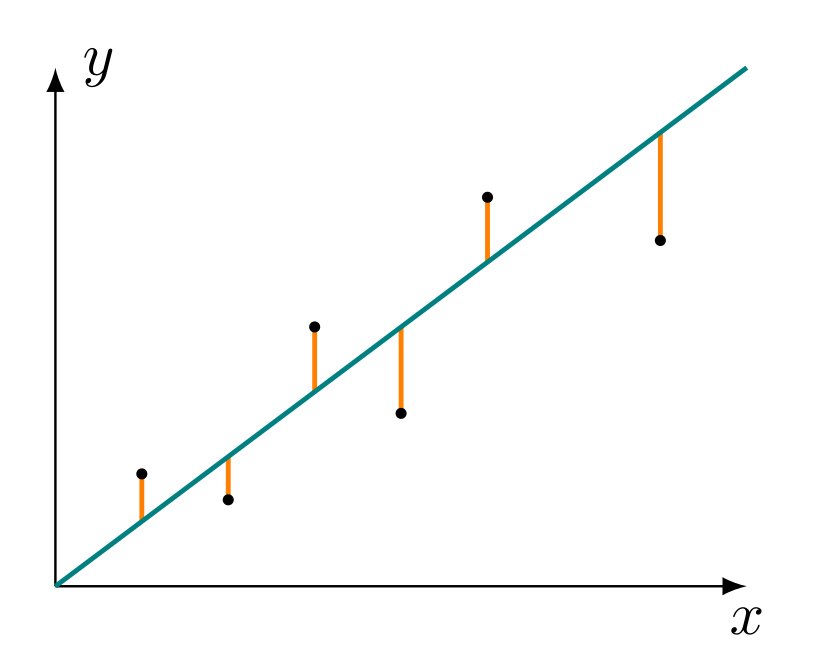
\includegraphics[width=0.4\textwidth]{figures/lsq.png}
    \caption{Classical Least-Squares Problem}~\label{fig:lsq}
\end{figure}

However, in many practical scenarios, the data matrix \(A\) and observation vector \(b\) may be subject to uncertainties or perturbations. The robust (or total) least-squares problem extends the classical formulation by considering these uncertainties, leading to a more resilient estimation process:
\[
\min_{\Delta A, \Delta b} \left\| \begin{bmatrix} \Delta A & \Delta b \end{bmatrix} \right\|_F^2
\quad\text{subject to}\quad
(A + \Delta A)x = b + \Delta b,
\]
where \(\Delta A\) and \(\Delta b\) represent the uncertainties in the data matrix and observation vector, respectively. The problem can be visualized in Figure~\ref{fig:total-lsq}. 

\begin{figure}[h]
    \centering
    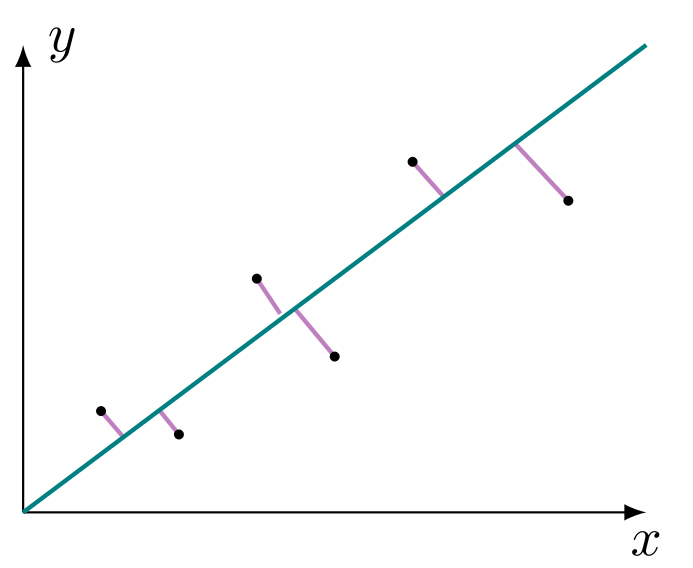
\includegraphics[width=0.4\textwidth]{figures/total-lsq.png}
    \caption{Total Least-Squares Problem}~\label{fig:total-lsq}
\end{figure}

Significant advancements have been made in solving robust least-squares problems, including the development of efficient algorithms and theoretical guarantees for their performance~\cite{ghaoui97}. This framework led to an equivalent reformulation of the robust least-squares problem as a minimax optimization problem, posed as:
\[\min_{x \in \mathbb{R}^n} \max_{A \in \B_{\rho}(\hat{A})} \|Ax - b\|_2^2,\]
where \(\B_{\rho}(\hat{A})\) denotes a ball of radius \(\rho\) centered at the nominal data matrix \(\hat{A}\). This reformulation allows for the application of bilevel optimization techniques to solve the robust least-squares problem efficiently, especially when $A$ has a special structure (e.g.\ elements on a manifold). The geometrically robust least-squares problem can be visualized in Figure~\ref{fig:robust-lsq}.

\begin{figure}[h]
    \centering
    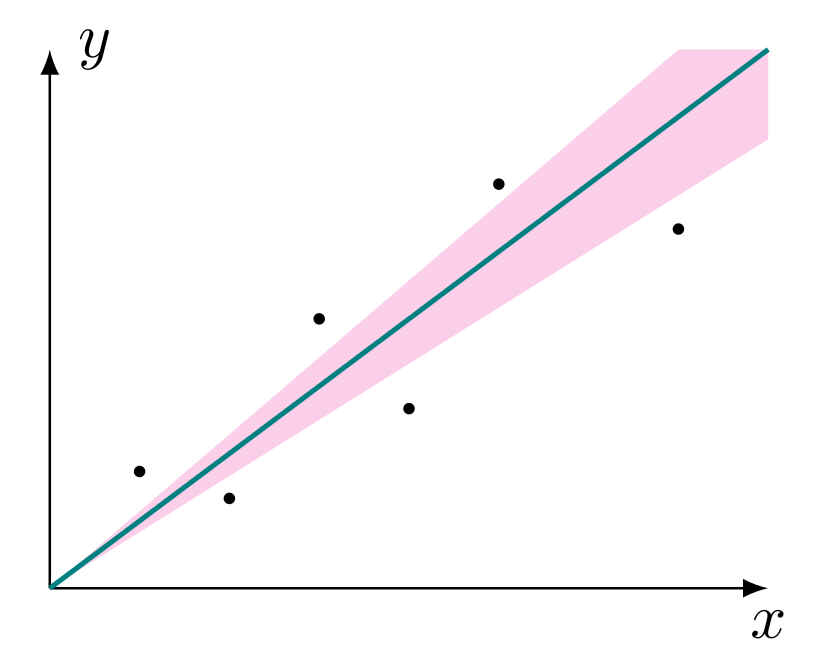
\includegraphics[width=0.4\textwidth]{figures/robust-lsq.png}
    \caption{(Geometrically) Robust Least-Squares}~\label{fig:robust-lsq}
\end{figure}

All these variants of least-squares problems indeed have explicit solutions that can be computed efficiently using singular value decomposition (SVD) techniques~\cite{golub1980}. However, in practice, we usually encounter constraints on the feasible set of solutions. This leads to constrained robust least-squares problems, which are generally more challenging to solve. Various approaches have been proposed to tackle these problems, including regularization, convex relaxation techniques, iterative algorithms, and heuristic methods.

\section{Behavioral Approach to System Theory}
The behavioral approach to system theory, pioneered by Jan C. Willems in the 1980s~\cite{willems1986}, provides a framework for modeling and analyzing dynamical systems based on their observed behaviors rather than traditional state-space representations. This approach emphasizes the importance of trajectories and the relationships between inputs and outputs, allowing for a more flexible and general representation of systems. The behavioral approach has been applied to various areas, including system identification, control design, and fault detection.

    \begin{figure}[h]
        \centering
        \begin{minipage}{0.32\textwidth}
            \centering
            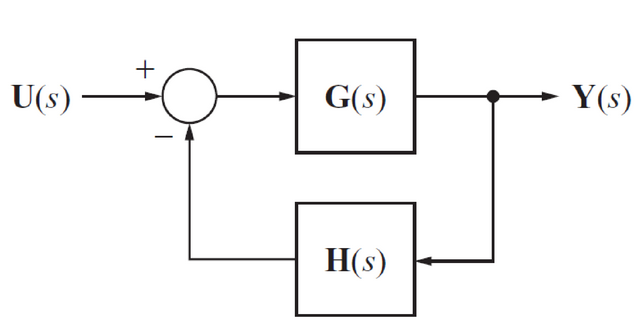
\includegraphics[width=\linewidth]{figures/transfer-function.png}
            \parbox{\linewidth}{\centering\small Transfer function}
            % \label{fig:placeholder}
        \end{minipage}\hfill
        \begin{minipage}{0.32\textwidth}
            \centering
            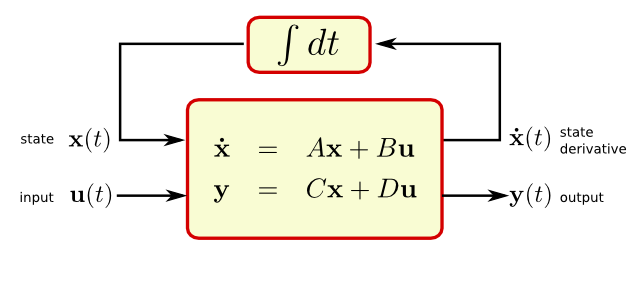
\includegraphics[width=\linewidth, trim={2cm, 0cm, 3cm, 0cm}, clip]{figures/state-space.png}
            \parbox{\linewidth}{\centering\small State-space}
            % \label{fig:placeholder}
        \end{minipage}\hfill
        \begin{minipage}{0.32\textwidth}
            \centering
            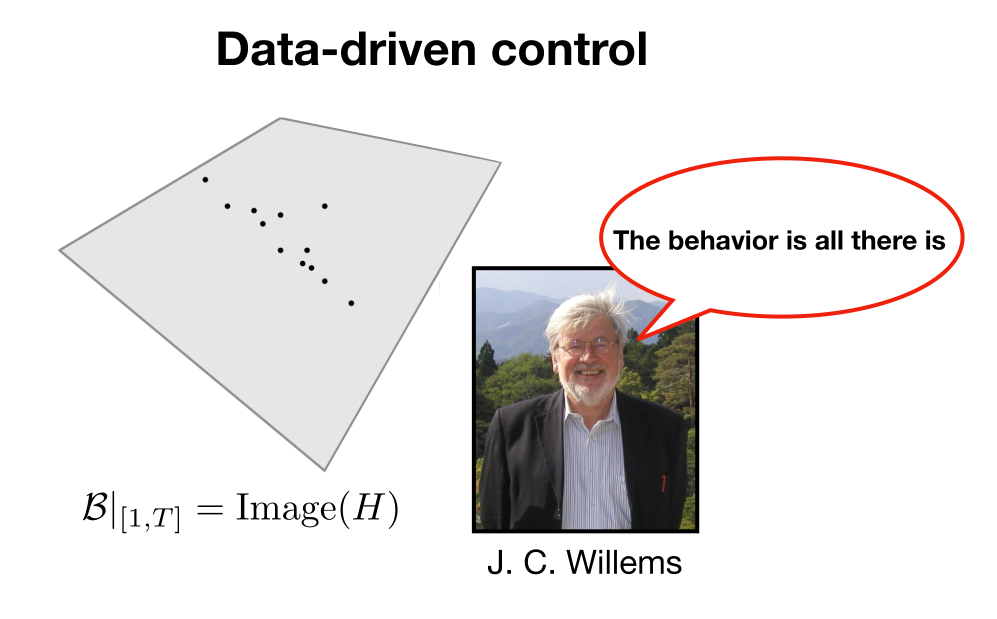
\includegraphics[width=\linewidth, trim={0cm 0cm 0cm 3cm}, clip]{figures/behavior.png}
            \parbox{\linewidth}{\centering\small Behavior}
            % \label{fig:placeholder}
        \end{minipage}
    \end{figure}

Willems' seminal work laid the foundation for the behavioral approach, introducing key concepts such as the notion of a system's behavior as a set of trajectories and the idea of controllability and observability in this context. Subsequent research expanded on these ideas, exploring various aspects of behavioral systems, including their interconnections, feedback control, and robustness properties~\cite{willems1989,padoan2022}.

\section{Data-Driven Control Methods}
Data-driven control methods have gained significant attention in recent years due to their ability to leverage data directly for control design, bypassing the need for explicit system identification. These methods are particularly useful in scenarios where obtaining accurate models is challenging or impractical. One prominent class of data-driven control methods is predictive control, which utilizes historical data to predict future system behavior and optimize control actions accordingly. Predictive control methods, such as Model Predictive Control (MPC), have been widely studied and applied in various domains, including process control, robotics, and autonomous systems~\cite{camacho2007}.

Recent advancements in data-driven predictive control via behavioral system theory have led to the development of novel control strategies that directly utilize input-output data for control synthesis. These approaches often involve constructing Hankel matrices from collected data and formulating optimization problems that ensure desired closed-loop properties, such as stability and performance. A notable example is the work by Coulson et al.~\cite{jeremy2019}, which introduced a data-driven predictive control (DeePC) framework based on Willems' fundamental lemma. This framework allows for the design of controllers that guarantee closed-loop stability and performance without requiring an explicit model of the system, including complex nonlinear systems like quadcopters.


